\documentclass[man, floatsintext]{apa7}
\usepackage[american]{babel}
\usepackage{csquotes}
\usepackage{amsmath,amsthm,bm,bbm,amsfonts,textcomp}
\usepackage[justification=centering]{subcaption}
\usepackage[justification=centering]{caption}
\usepackage[style=apa, backend=biber]{biblatex}
\addbibresource{lit.bib}

\title{Conditionally Unbiased Best Linear Predictors for Score Augmentation}
\shorttitle{Score augmentation using CUBLP}
\authorsnames{Xiang Liu, Matthew S. Johnson, Sandip Sinharay}
\authorsaffiliations{Educational Testing Service}

%% new commands %%
\newcommand{\mbf}[1]{\bm{#1}}
\newcommand{\bc}{\mbf{c}}
\newcommand{\bX}{\mbf{X}}
\newcommand{\bY}{\mbf{Y}}
\newcommand{\bT}{\mbf{T}}
\newcommand{\C}{\mathcal{C}}
\newcommand{\bbeta}{\mbf{\beta}}
\newcommand{\bmu}{\mbf{\mu}}
\newcommand{\beps}{\mbf{\varepsilon}}
\newcommand{\btau}{\mbf{\tau}}
\newcommand{\bgamma}{\mbf{\gamma}}
\newcommand{\blambda}{\mbf{\lambda}}
\newcommand{\bW}{\mbf{W}}
\newcommand{\bsigma}{\mbf{\Sigma}}
\newcommand{\E}{\mathbb{E}}
\newcommand\independent{\protect\mathpalette{\protect\independenT}{\perp}}
\def\independenT#1#2{\mathrel{\rlap{$#1#2$}\mkern2mu{#1#2}}}
\DeclareMathOperator{\MSE}{MSE}
\DeclareMathOperator{\Cov}{Cov}
\DeclareMathOperator{\Var}{Var}
%%%%%%%%%%% 

\abstract{The best linear predictor (BLP) has been proposed to combine
different types of information in estimating true scores. The BLP is
biased for individual examinees when conditioned on the true score. In this
paper, we propose a conditionally unbiased BLP. Additionally, a least square
method is introduced for parameter estimation.}

\begin{document}
  \maketitle

  \section{Introduction}
	With the current popular trend of transition from traditional paper-pencil
  assessments to digital formats, an increasingly common task is to combine
  different sources of information in assessing some latent construct. For
  instance, in the context of writing assessments, in addition to the final
  product essays, digital platforms are now able to capture information on
  keystrokes during
  students' interaction with writing tasks. Thus, features related to writing
  process are now becoming available (e.g. \cite{Zhang2019,Guo2019}).
  Furthermore, additional product features such as those related to natural
  language processing (NLP) could also be obtained through NLP programs (e.g.
  the e-rater\textsuperscript{\textregistered} program; 
  \cite{Attali2006,Burstein2004}). Then a natural question is whether and how
  different sources of information can be combined to augment the rater
  scores in making inferences on examinees' writing proficiency.

  There has been some previous research exploring related methods. For example,
  \textcite{Zhang2015} used linear regression to predict adjudicated essay
  scores from a large number of keystroke logging features and other product
  features. \textcite{Sinharay2019} examined the same prediction problem
  utilizing machine learning methods such as the random forests and boosting. A
  common assumption of these methods is that essay score, the prediction
  target, is treated as fixed and known. However, in educational and
  psychological measurement, prediction targets are almost always latent and
  measured with error. To address this issue, the best linear predictors (BLP;
  e.g. \cite{Haberman2015,Yao2019}) has been proposed to combine sources of
  information (e.g. scores from other sections) along with manifest variables
  such as the rater scores to predict some latent true score (e.g. the
  writing proficiency). It should be noted that, due to some historical reasons,
  in the field of animal breeding where the methods of BLP and BLUP were first
  popularized, random effects are said to be "predicted" as opposed to be
  "estimated" for fixed effects. However, in our field of psychometrics and
  educational/psychological measurement, such distinction is not customary.
  Thus both terms, prediction and estimation, are used synonymously and
  interchangeably in this paper.

  The BLP minimizes the mean squared error (MSE) of prediction among all linear
  predictors. An important property of the BLP is that, when averaged over the
  population, the expected prediction is equal to the expected true score. In
  other words, the BLP is unbiased. However, it exhibits shrinkage towards
  the population mean. Consequently, the BLP is biased conditional on the true
  score level \parencite{Robinson1991}. This may lead to some serious fairness
  concern as the BLP could favor certain groups of examinees over others.

  In this paper, we introduce a conditionally unbiased best linear predictor 
  (CUBLP) for estimating latent variable from multiple sources that minimizes
  the prediction error among all linear predictors that are unbiased at all true
  score levels. The proposed method is flexible and can be applied to a wide
  variety of problems.

  \section{Methods}
  Let $\bW = (\bY^\top, \bX^\top)^\top$ denote observed random variables
  from a random examinee where $\bY = (Y_1, Y_2, \dots, Y_J)^\top$ is the vector
  of variables measured with error (commonly referred to as manifest
  variables of some latent trait, e.g. essay scores from raters).
  and $\bX = (X_1, X_2, \dots, X_K)^\top$ is the vector of variables measured
  without error (i.e. covariates that may correlate with the latent
  trait of interest, e.g. typing speed).  For simplicity, we consider an
  unidimensional latent true score $S$ and further assume that $\bW$ and $S$ are
  linearly related, i.e.
  \begin{equation}
    \mbf{W} = \left (
      \begin{array}{c} \bY \\  \bX \end{array} \right ) =
    \mbf{\alpha} + \mbf{\lambda} S + \mbf{\varepsilon}_w.
  \end{equation}
  It is mathematically more convenient and simplifies discussions when $\bW$ is
  centered, $E[\bW] = 0$, which leads to
  \begin{equation}
  \label{eq:linear_model}
    \bW = \blambda S + \mbf{\varepsilon}_w.
  \end{equation}
  For identifiability, the following constraints are imposed, $\E(S) = 0$ and
  $\E(\beps_w) = \mbf{0}$. Furthermore, the variance-covariance matrix of the
  random effects, the latent variable $S$ and the residuals $\beps_w$, is in the
  form
  \begin{equation}
    \Cov\left(\begin{array}{c} S \\ \beps_w \end{array}\right) = \begin{bmatrix}
      \sigma_S^2 & 0 \\
      0 & \bsigma_{\beps_w}
    \end{bmatrix}.
  \end{equation}
  In other words, the cross-covariance of $S$ and $\beps_w$ is zero, i.e.
  $\Cov(S, \varepsilon_{w_i}) = 0, \forall i$.
  Notice that, similar to \textcite{Haberman2015}, we do not assume a specific
  structure for the variance-covariance matrix of the residuals, $\bsigma_
  {\beps_w}$. Thus, depending on the structure of $\bsigma_{\beps_w}$,
  Equation~\ref{eq:linear_model} describes a broad class of models (see
  Figure~\ref{fig:PGM_example} for examples).
  \begin{figure}[t]
    \begin{subfigure}[b]{0.45\textwidth}
      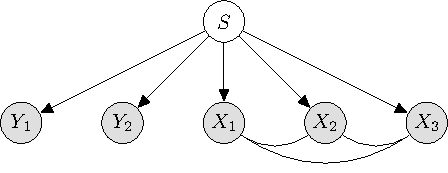
\includegraphics[width=\textwidth]{fig/model_1.pdf}
      \caption{Correlated residuals of $X$}
    \end{subfigure}\hfill
    \begin{subfigure}[b]{0.45\textwidth}
      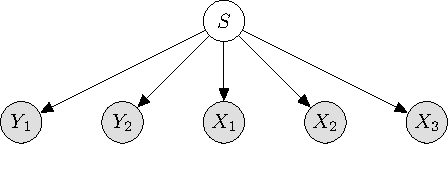
\includegraphics[width=\textwidth]{fig/model_2.pdf}
      \caption{Uncorrelated residuals of $X$}
    \end{subfigure}
    \caption{Graphical representation of some example models}
    \label{fig:PGM_example}
  \end{figure}
  For almost all real applications, we are interested in estimating the latent
  score $S$ from the observed random variables with some estimator, $\hat{S} = g
  (\bW)$.

  \subsection{The best linear predictors}
  The BLP estimator approaches the estimation problem by finding a linear
  combination of the observed random variables, $\hat{S} = \bgamma_1^\top
  \bW$, such that the mean squared error for prediction,
  \begin{equation}
  \label{eq:MSE}
    \MSE = E[(S - \bgamma_1^\top \bW )^2],
  \end{equation}
  is minimized. The MSE can be expanded as
  \begin{align}
    \MSE &= E[S^2 + (\bgamma_1^\top \bW)^2 - 2S\bgamma_1^\top \bW]\\
    &= E[S^2] + E[(\bgamma_1^\top \bW)^2] - 2\bgamma_1^\top E[S\bW]\\
    &= \sigma_S^2 + \Var(\bgamma_1^\top \bW) - 2\bgamma_1^\top E[\blambda S^2 +
    S\mbf{\varepsilon}_w]\\
    &= \sigma_S^2 + \bgamma_1^\top \bsigma_{\bW} \bgamma_1 - 2\bgamma_1^\top
    \blambda \sigma_S^2,
  \end{align}
  where $\Sigma_{\bW}$ is the variance-covariance matrix of the observed random
  variables $\bW$.
  From Equation 7 to Equation 8, we assume $E[\mbf{\varepsilon}_w|S] = 0$,
  thus $E[S\mbf{\varepsilon}_w] = E[S E(\mbf{\varepsilon}_w|S)]$ = 0. Solving
  the gradient function with respect to $\blambda_1$,
  \begin{align}
    \nabla \MSE &= \nabla(\bgamma_1^\top \bsigma_{\bW} \bgamma_1)  - \nabla
    (2\bgamma_1^\top \blambda \sigma_S^2) \\
    &= 2\Sigma_{\bW} \bgamma_1 - 2 \blambda \sigma_S^2 = 0,
  \end{align}
  leads to the BLP coefficient $\bgamma_1 = \Sigma_{\bW}^{-1} \blambda
  \sigma_S^2$.
  Therefore, the BLP estimator of the latent score is $\hat{S} = (\Sigma_{\bW}^
  {-1} \blambda\sigma_S^2)^\top \bW$. The model in Equation 
  \ref{eq:linear_model} and its associated assumptions imply that the
  variance-covariance matrix of $\bW$ can be decomposed as
  \begin{equation}
  \label{eq:cov_decomp}
    \Sigma_{\bW} = \sigma_S^2\blambda\blambda^\top + \bsigma_{\mbf{\varepsilon}_w}.
  \end{equation}
  By the Woodbury matrix identity \parencite{Fill1999}, this decomposition of
  $\Sigma_{\bW}$ leads to an alternative expression of the BLP coefficients,
  \begin{equation}
    \bgamma_1 = \frac{\Sigma_{\mbf{\varepsilon}_w}^{-1}\blambda}{1/\sigma_S^2 +
    \blambda^\top\Sigma_{\mbf{\varepsilon}_w}^{-1}\blambda}.
  \end{equation}

  The bias of the BLP in estimating $S$ is
  \begin{align}
    Bias(\hat{S}) &= E[\hat{S} - S] \\
    &= E[(\sigma_S^2\blambda^\top \Sigma_{\bW}^{-1})\bW - \lambda^{-1}\bW +
    \blambda^{-1}\mbf{\varepsilon}_w] \\
    &= \sigma_S^2\blambda^\top \Sigma_{\bW}^{-1} E[W] - \blambda^{-1}E[\bW] +
    \blambda^{-1}E[\mbf{\varepsilon}_w] = 0.
  \end{align}
  In other words, when averaged over the entire population, the BLP is unbiased
  in estimating $S$.

  \subsection{The conditional bias of the BLP}
  We showed that the BLP is marginally unbiased. However, there is no
  guarantee that it has the same unbiasedness property for each individual. To
  assess the bias for estimating the latent true score for each individual, we
  need to evaluate the bias of the BLP conditional on latent true score levels,
  i.e.
  \begin{align}
    E[\hat{S} - S|S] &= E[\sigma_S^2\blambda^\top\Sigma_{\bW}^{-1}\bW|S] - S
    \nonumber\\
    &= E[\sigma_S^2\blambda^\top\Sigma_{\bW}^{-1}(\blambda S + 
    \mbf{\varepsilon}_w)|S] - S \nonumber\\
    &= \sigma_S^2\blambda^\top\Sigma_{\bW}^{-1}\blambda S - S \nonumber\\
    &= S(\sigma_S^2\blambda^\top\Sigma_{\bW}^{-1}\blambda - 1). 
    \label{eq:conditional_bias}
  \end{align}

  Equation \ref{eq:conditional_bias} is illuminating that the conditional bias
  depends on two factors - the latent true score level $S$, and the ratio to
  which the total variance-covariance in the manifest variables can be explained
  by the latent true score. The conditional bias of the BLP is zero for all
  latent score levels $S = s, \forall s \in \mathbb{R}$ if and only if
  $\sigma_S^2\blambda^\top\Sigma_{\bW}^\top\blambda = 1$. That is, the latent
  true score $S$ perfectly explains the variance-covariance of the observed
  random variables $\Sigma_{\bW}$. But, for almost all realistic applications,
  this perfect relationship is rarely attainable. Thus, given a model, the
  estimation bias of the BLP is inversely proportional to the true score level
  for any individual.
  \begin{figure}[t]
  \centering
    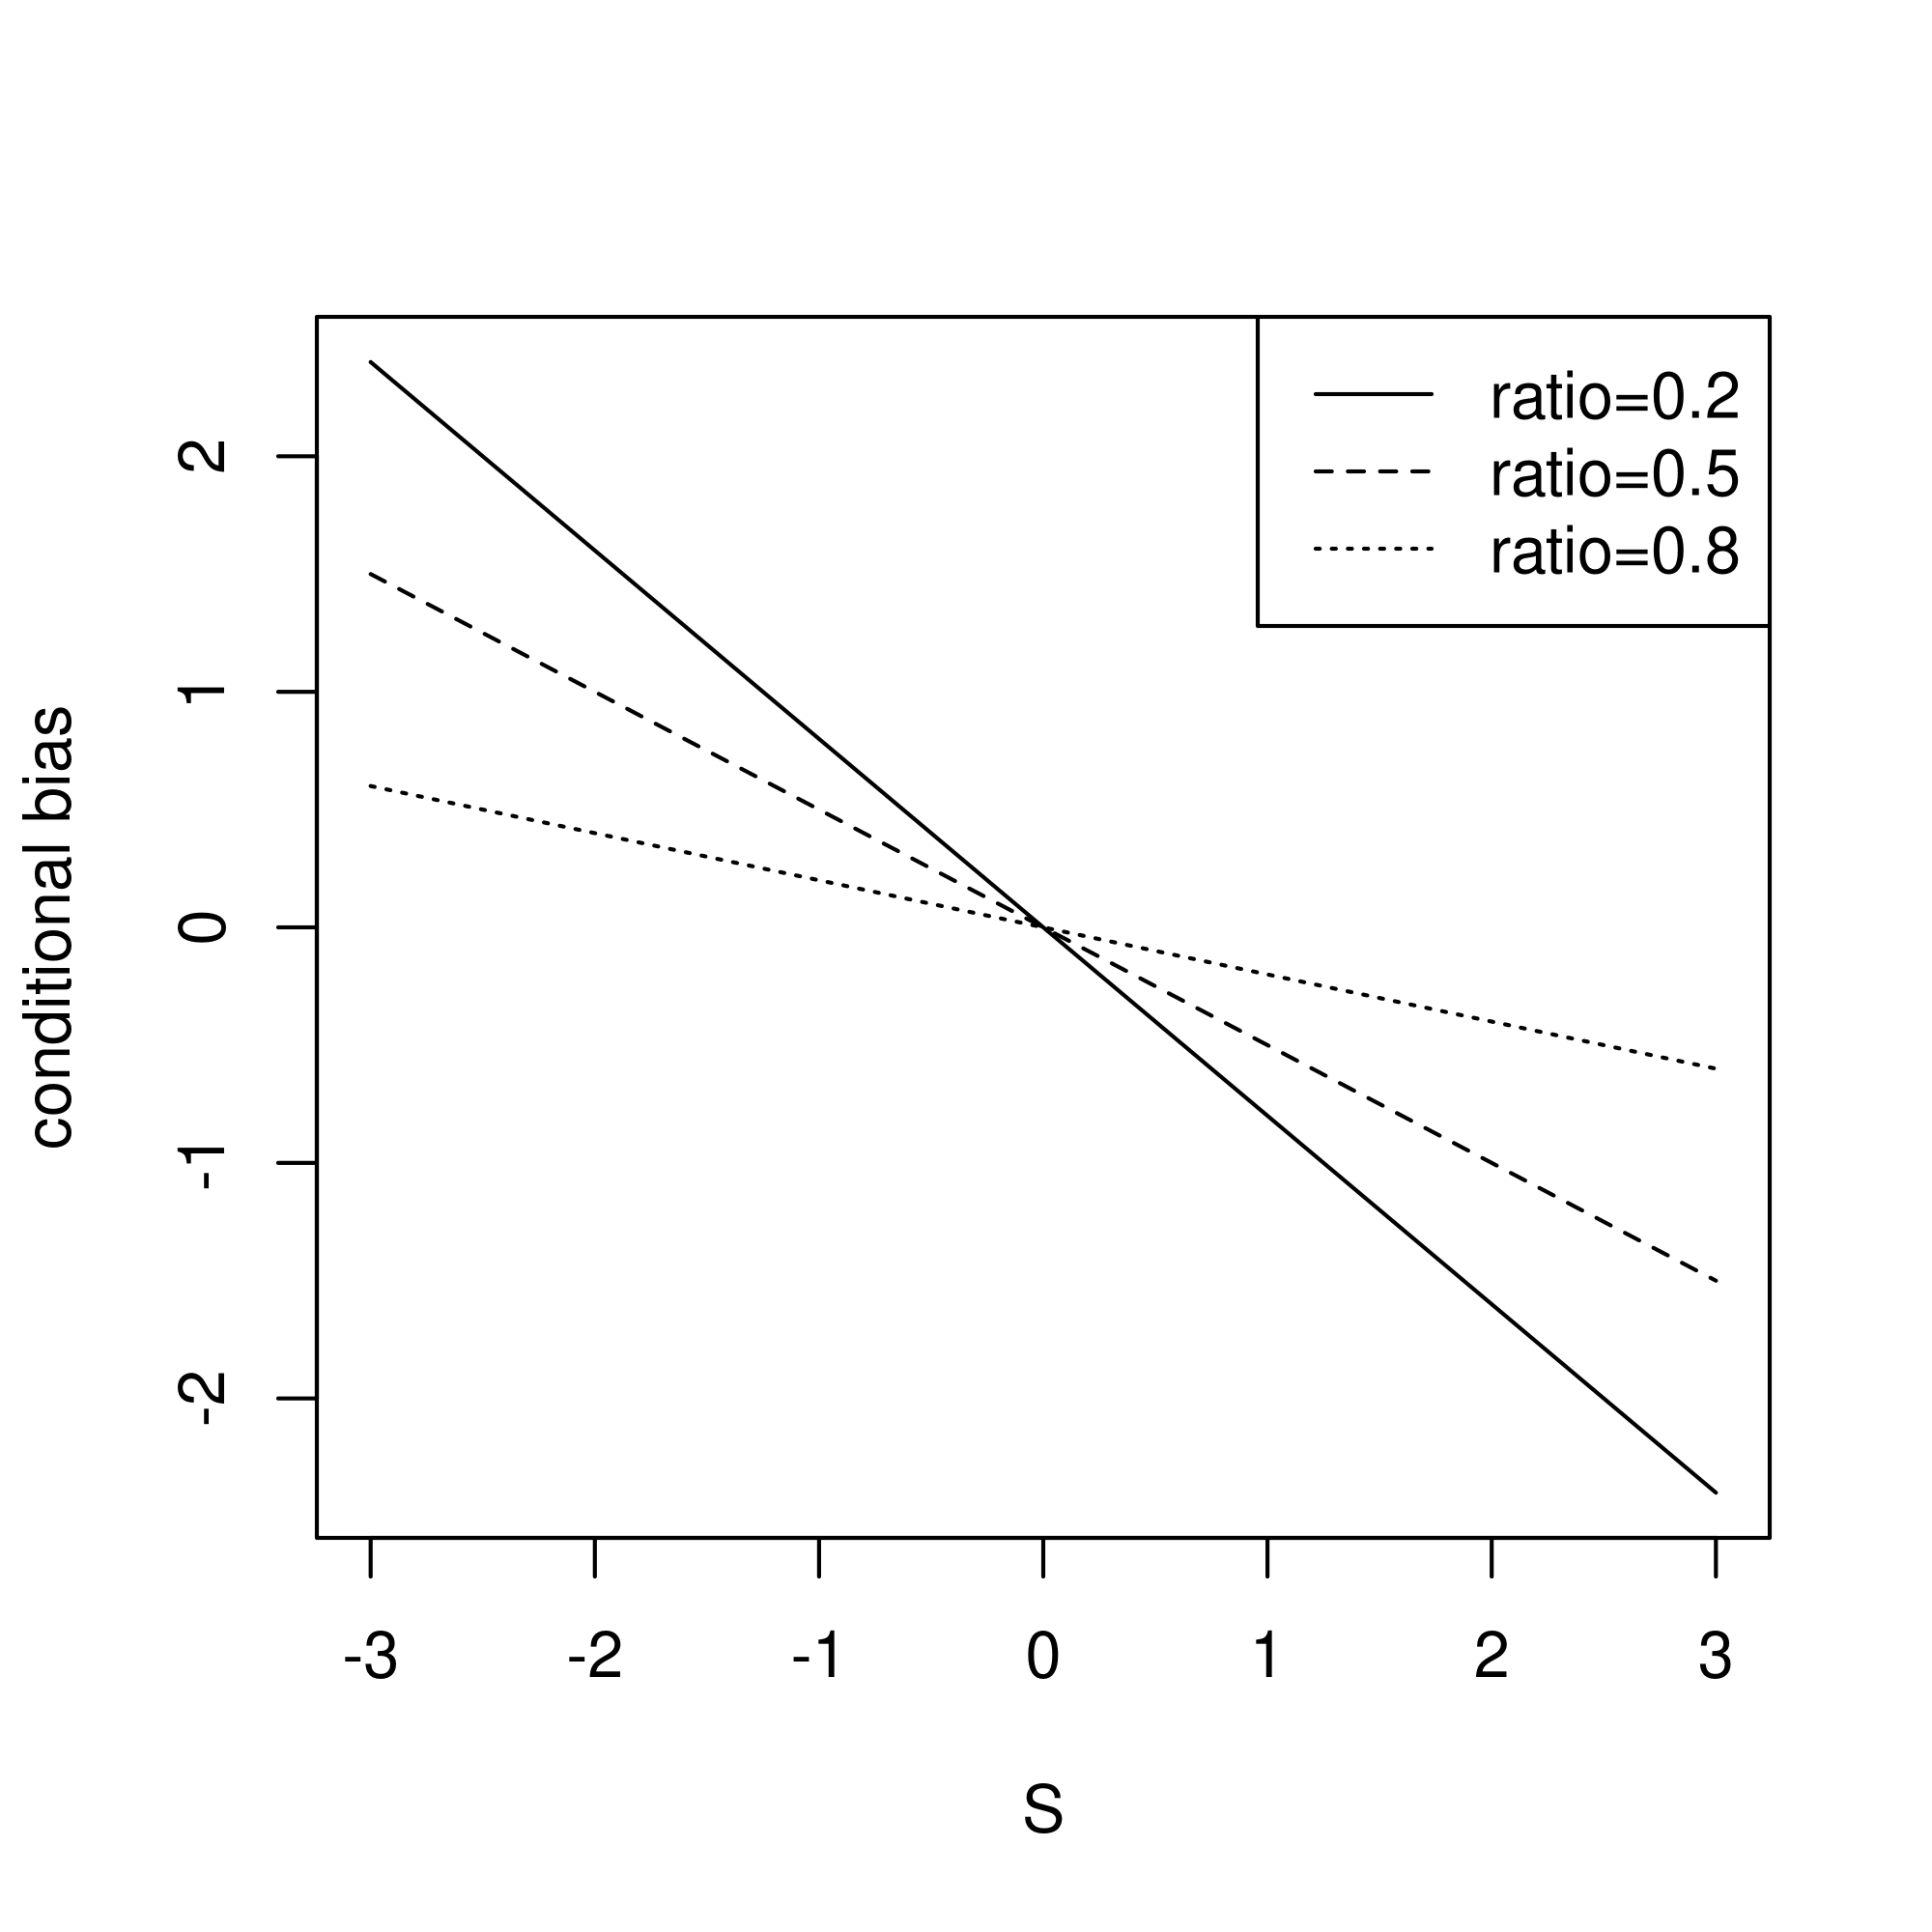
\includegraphics[scale = 0.65]{fig/conditional_bias.png}
    \caption{Conditional bias under different covariance ratios}
    \label{fig:conditional bias}
  \end{figure}
  Figure \ref{fig:conditional bias} illustrates the conditional bias of the
  BLP across levels of $S$ under low, medium, and high variance-covariance
  ratios. While the BLP is less biased in the medium level of $S$, it is
  positively biased for individuals with lower levels of the latent true score
  and negatively biased for those with higher levels of the latent true score.
  The demonstrated conditional bias of the BLP estimator may create threats to
  fairness and equity.

  \subsection{Conditionally unbiased BLP}
  To mitigate the potential threats to fairness and equity from conditional bias
  of BLP, we develop a conditionally unbiased BLP. Instead of finding the linear
  predictor, $\hat{S} = \bgamma_1^\top \bW$, which simply minimizes the MSE for
  prediction as in Equation~\ref{eq:MSE}, the CUBLP is further subject to a
  constraint that it is conditionally unbiased, i.e.
  \begin{equation}
    E[\bgamma_1^\top\bW|S] = \bgamma_1^\top E[\bW|S] = \bgamma_1^\top (\blambda
    S + E[\mbf{\varepsilon}_w|S]) = S.
  \end{equation}
  With the additional assumption that $E(\mbf{\varepsilon}_w|S) = 0$, the
  constraint simplifies to
  \begin{equation}
  \label{eq:unbias_constraint}
    \bgamma_1^\top \blambda = 1.
  \end{equation}
  It follows that the CUBLP coefficients can be found by minimizing $\MSE = E[
  (S-\bgamma_1^\top \bW)^2]$, subject to the constraint $\bgamma_1^\top
  \blambda = 1$. This constrained optimization problem can be solved by using
  the method of Lagrange multipliers. The Lagrange function is defined as
  \begin{equation}
    \mathcal{L} (\blambda_1, \delta) = -E[(S-\bgamma_1^\top \bW)^2] - \delta
    (\bgamma_1^\top \blambda - 1),
  \end{equation}
  where the Lagrange multiplier $\delta$ is a constant that ensures the
  constraint is met. The CUBLP coefficients $\blambda_1$ is found by solving
  \begin{equation}
    \nabla_{\blambda_1, \delta} \mathcal{L}(\blambda_1^\top, \delta) = \mbf{0},
  \end{equation}
  which is equivalent to solving the system of equations
  \begin{equation}
    \begin{cases}
      -2\bsigma_{\bW} \bgamma_1 + 2\blambda\sigma_S^2 = \delta\blambda\\
      \bgamma_1^\top \blambda -1 = 0
    \end{cases}.
  \end{equation}
  The solution leads to the CUBLP coefficients
  \begin{equation}
    \blambda_1 = \frac{\bsigma_{\bW}^{-1}\blambda}{\blambda^\top \bsigma_{\bW}^
    {-1}\blambda}.
  \end{equation}
  Using the covariance matrix decomposition in Equation~\ref{eq:cov_decomp} and
  the Woodbury matrix identity, it is straightforward to verify that the CUBLP
  coefficients can be alternatively expressed in terms of the residual
  covariance matrix,
  \begin{equation}
    \blambda_1 = \frac{\bsigma_{\mbf{\varepsilon}_w}\blambda}{\blambda^\top
    \bsigma_{\mbf{\varepsilon}_w} \blambda}.
  \end{equation}

  \subsection{Parameter estimation}
  Notice that the derived BLP and CUBLP coefficients are expressed as a function
  of the population parameters $\blambda$, and $\Sigma_{\bW}$ or $\mbf{\Sigma}_
  {\beps_w}$. In other words, they are treated as known. However, in most
  applications, these quantities would have to be estimated. We derive a least
  square estimator for the parameters in this section.

  Let \[ \blambda = \left (\begin{array}{r} \blambda_{\bY} \\ \blambda_{\bX} 
  \end{array} \right) \], where $\blambda_{\bY} = (\lambda_{Y_1}, \lambda_{Y_2},
  \dots, \lambda_{Y_K})'$ and $\blambda_{\bX} = (\lambda_{X_1}, \lambda_{X_2},
  \dots, \lambda_{X_J})'$.
  Assume all observed variables are standardized and $E(S) = \mu_S = 0$ and
  $\sigma^2_{S} = 1$. It leads to
  \begin{equation}
  \mbf{\Sigma}_{\bW} = \blambda \blambda^\top + \mbf{\Sigma}_{\beps}.
  \end{equation}
  We further assume that the covariance of $\bY$ is fully explained by $S$. That
  is
  \begin{equation}
    \mbf{\Sigma}_{\bY} = \blambda_{\bY} \blambda_{\bY}^\top + \mbf{\Psi}_{\bY},
  \end{equation}
  where $\mbf{\Psi}_{\bY}$ is a diagonal matrix with residual variances of $\bY$
  on the main diagonal. This is a common assumption for many popular measurement
  models. Now, we impose some additional restrictions on the residual covariance
  matrix $\mbf{\Sigma}_{\beps}$. $\bY$ is assumed to be uncorrelated with $\bX$
  given S. Equivalently, $\Cov(\beps_{\bY}, \beps_{\bX}) = \mbf{0}$.

  In many cases, it may be desirable or necessary to assume that $\lambda_{Y_j}
  = \lambda_{Y}$, $\forall j$. This equal discrimination assumption also
  simplifies the estimation of $\blambda$. Consider a quadratic loss function,
  \begin{equation}
    L(\blambda) = \sum_{k \neq k'} (\lambda_{Y}^2 - r_{Y_k Y_{k'}})^2 + \sum_k
    \sum_j (\lambda_Y \lambda_{X_j} - r_{Y_k X_j})^2,
  \end{equation}
  where $r_{m, n}$ denotes the observed correlation between random variables $m$
  and $n$. Taking the gradient to minimize the loss function,
  \begin{equation}
  \label{eq:loading_gradient_eqs}
    \nabla L = \left(
    \begin{array}{c} 4\lambda_Y \sum_{k \neq k'}(\lambda_{Y}^{2} - r_{Y_k Y_
    {k'}}) + 2K\lambda_Y\sum_j\lambda_{X_j}^2 - 2\sum_j \lambda_{X_j} \sum_k r_
    {Y_k X_j}\\
    \vdots\\
    2K\lambda_Y^2\lambda_{X_j} - 2\lambda_Y\sum_k r_{Y_k X_j}\\
    \vdots
    \end{array}\right) = \mbf{0}.
  \end{equation}
  Solving Equation \ref{eq:loading_gradient_eqs} leads to the unweighted least
  square estimator of the loadings,
  \begin{equation}
    \hat{\lambda_Y} = \sqrt{\frac{\sum_{k \neq k'} r_{Y_k Y_{k'}}}{K(K-1)}}
  \end{equation}
  and
  \begin{equation}
    \hat{\lambda_{X_j}} = \frac{\sum_k r_{Y_k X_j}}{K\hat{\lambda_Y}}.
  \end{equation}

  For unequal discrimination cases, the LS estimator can be obtained by
  iterating through
  \begin{equation}
    \hat{\lambda_{Y_k}} = \frac{\sum_{k' \neq k} \lambda_{Y_{k'}} r_{Y_{k}Y_
    {k'}} + \sum_j \lambda_{X_j} r_{Y_k, X_j}}{\sum_{k' \neq k} \lambda_{Y_
    {k'}}^2 + \sum_j \lambda_{X_j}^2},
  \end{equation}
  and
  \begin{equation}
    \hat{\lambda_{X_j}} = \frac{\sum_k \lambda_{Y_k} r_{Y_k X_j}}{\sum_k
    \lambda_{Y_k}^2}
  \end{equation}
  until convergence. 

  Without any parametric distribution assumption on the data, the covariance
  matrix $\bsigma_{\bW}$ is commonly estimated by the sample covariance matrix,
  \begin{equation}
    \hat{\bsigma_{\bW}} = \frac{1}{N-1}\sum_{i = 1}^{N}(\bW_{i} - \bar{\bW})
    (\bW_{i} - \bar{\bW})^\top,
  \end{equation} 
  where $N$ is the number of observations. If a multivariate Gaussian assumption
  is reasonable, the ML may be preferred, i.e.
  \begin{equation}
    \hat{\bsigma_{\bW}} = \frac{1}{N}\sum_{i = 1}^{N}(\bW_{i} - \bar{\bW})
    (\bW_{i} - \bar{\bW})^\top.
  \end{equation}
  A natural choice of an estimator for the residual covariance matrix is then 
  \begin{equation}
    \hat{\mbf{\Sigma}_{\beps_w}} = \hat{\mbf{\Sigma}_{\bW}} - \hat{\blambda} 
    \hat{\blambda}^\top.
  \end{equation}
  By substituting the population parameters with their estimates from the data,
  the BLP and CUBLP estimators become the empirical BLP and CUBLP estimators.

  \section{Simulations}
  \subsection{Properties of the LS estimator}
  We do not formally investigate the theoretical properties of the LS estimator
  in this paper. However, a small simulation is provided here to offer some
  empirical evidence of their properties. 

  The loadings are fixed as $\blambda = (0.8, 0.7, 0.6, 0.3)$. True scores $S$
  are randomly drawn from a standard normal distribution. Residuals
  $\mbf{\varepsilon}_{\bW}$ are generated from a multivariate normal
  distribution, $N(\mbf{0}, \bsigma_{\mbf{\varepsilon}_{\bW}}$) where the
  covariance matrix $\bsigma_{\mbf{\varepsilon}_{\bW}} = \mathbb{I} - \blambda
  \blambda^\top$. The observations $\bW$ are then computed according to the
  model in Equation~\ref{eq:linear_model}. Using the generated data $\bW$, the
  loadings are estimated using the least square method. 

  Figure~\ref{fig:ls_bias_var} shows the bias and the variance of the LS
  estimator over 1000 replications for varying sample sizes.
  \begin{figure}[t]
    \centering
    \begin{subfigure}[b]{0.45\textwidth}
      \centering
      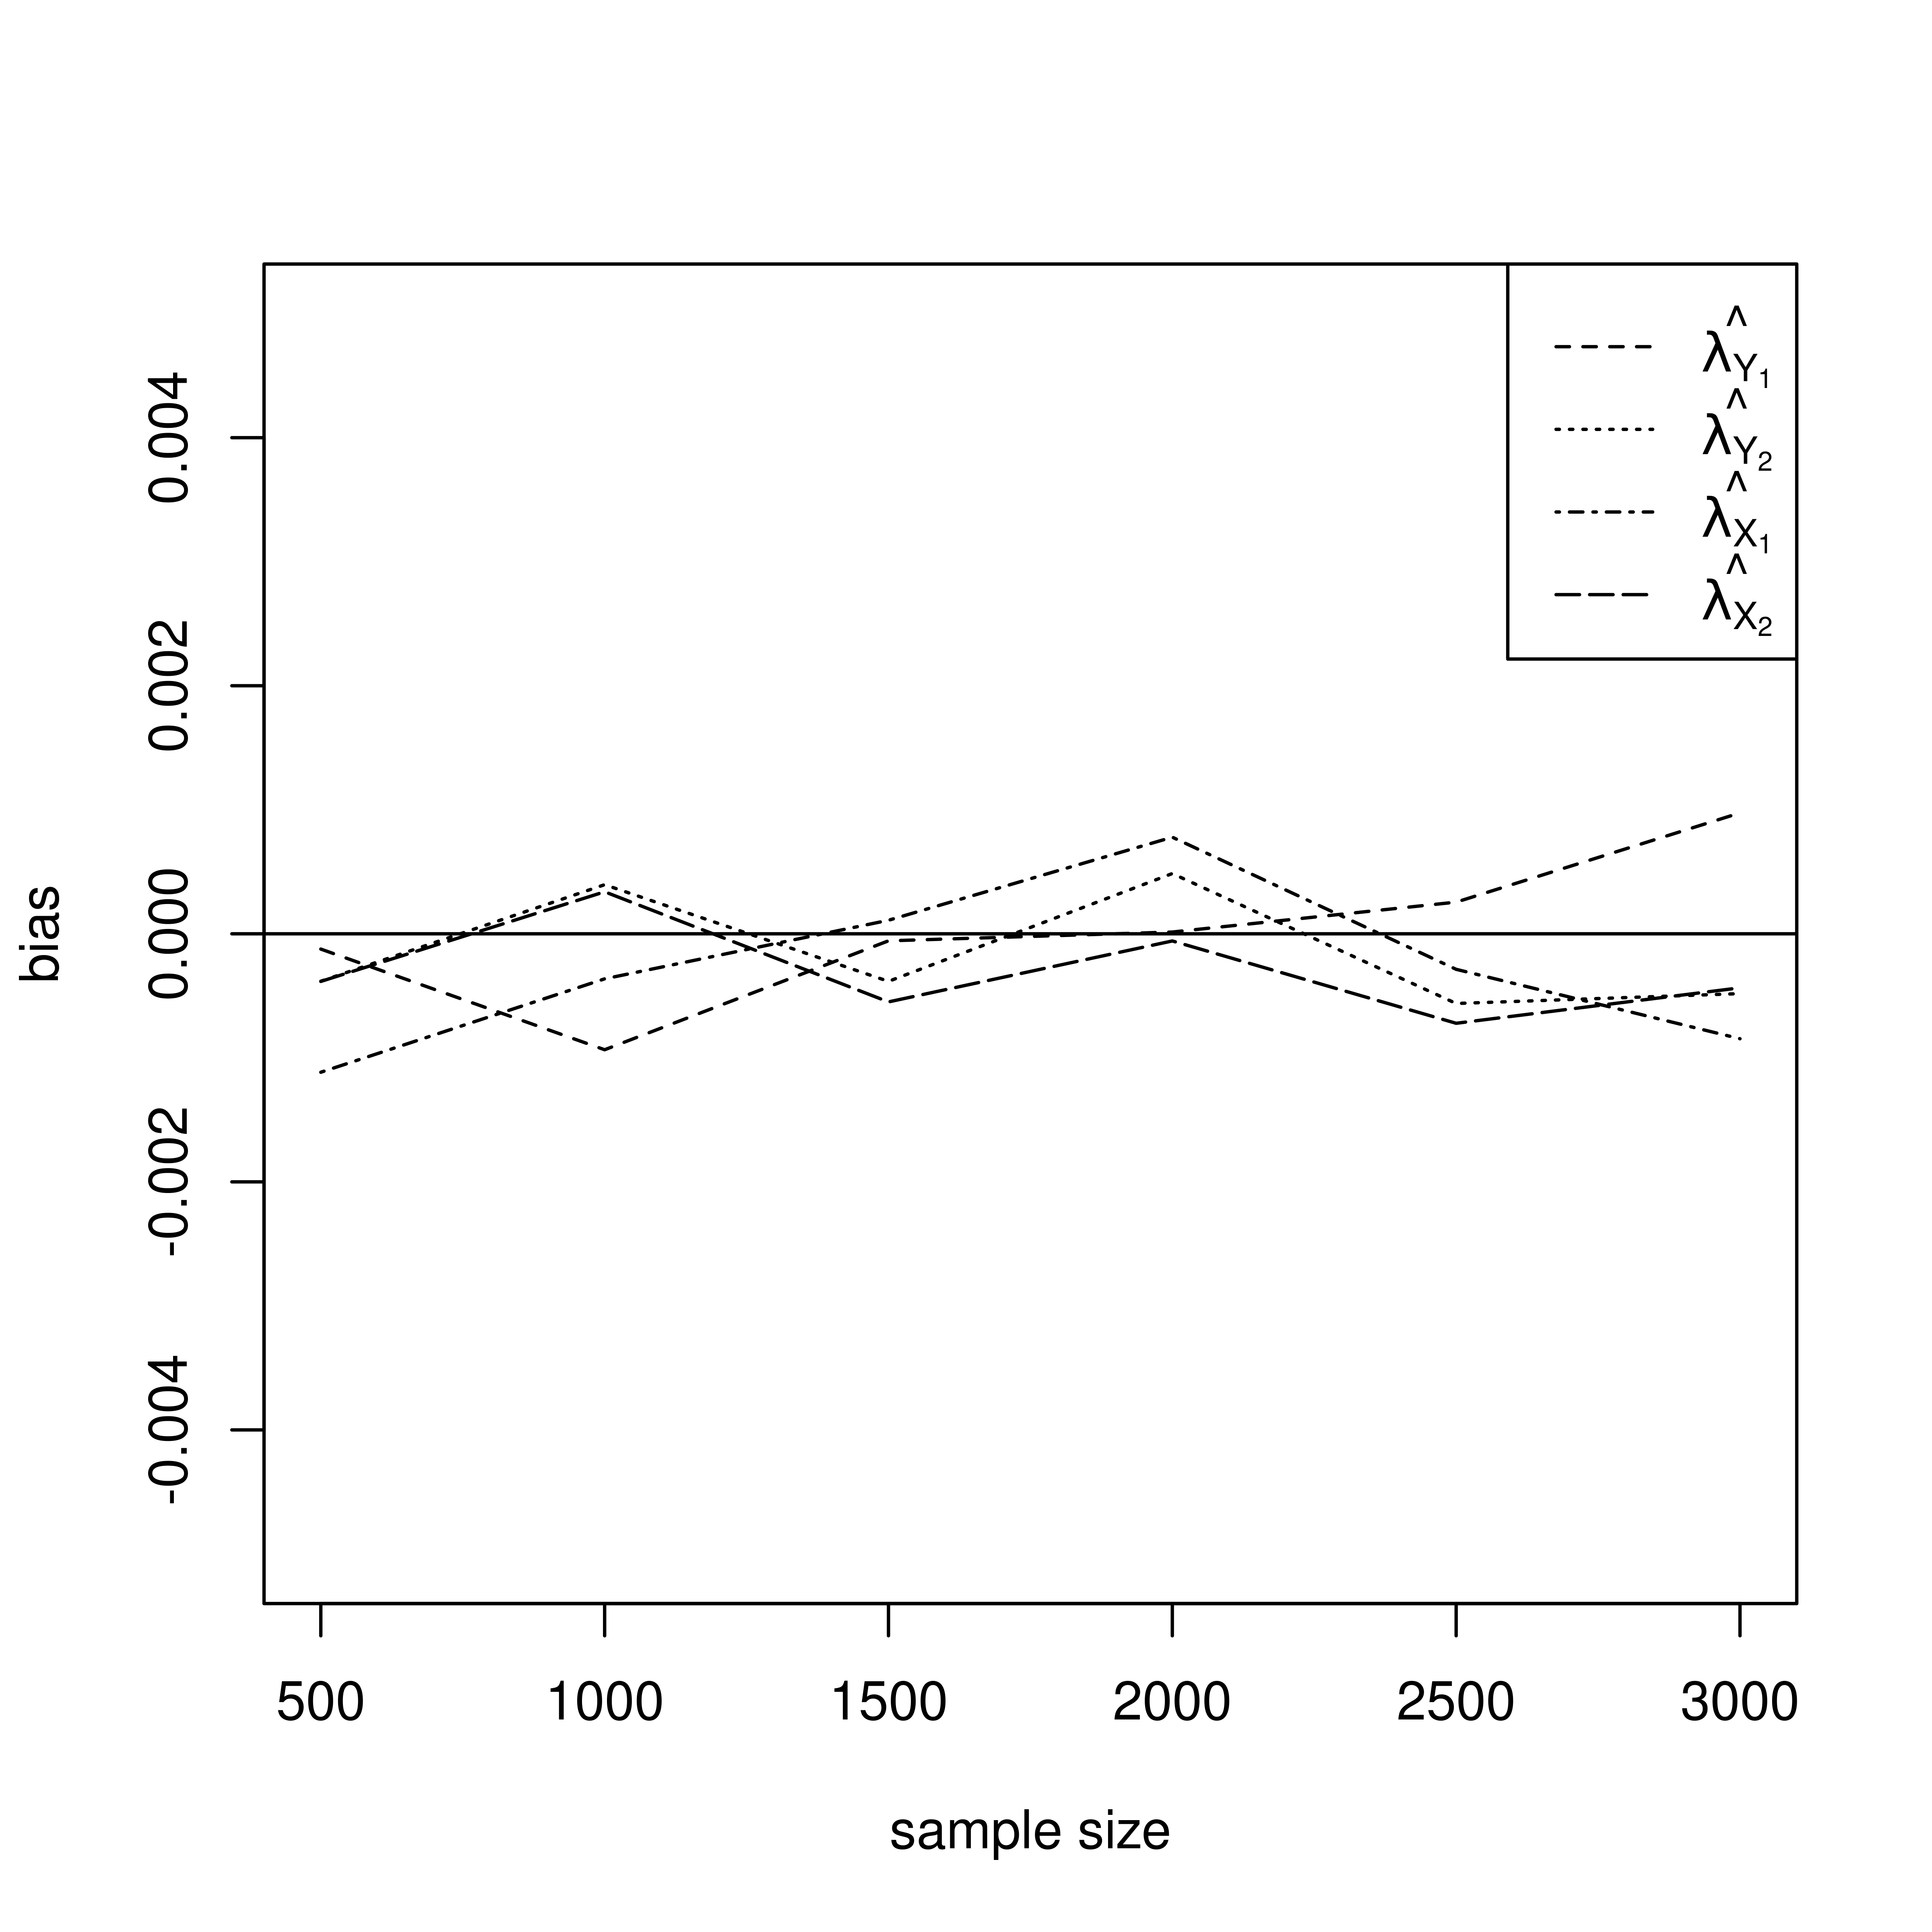
\includegraphics[width=\textwidth]{fig/bias_uneq_discrim_high.png}
      \caption{Bias}
    \end{subfigure}
    \begin{subfigure}[b]{0.45\textwidth}
      \centering
      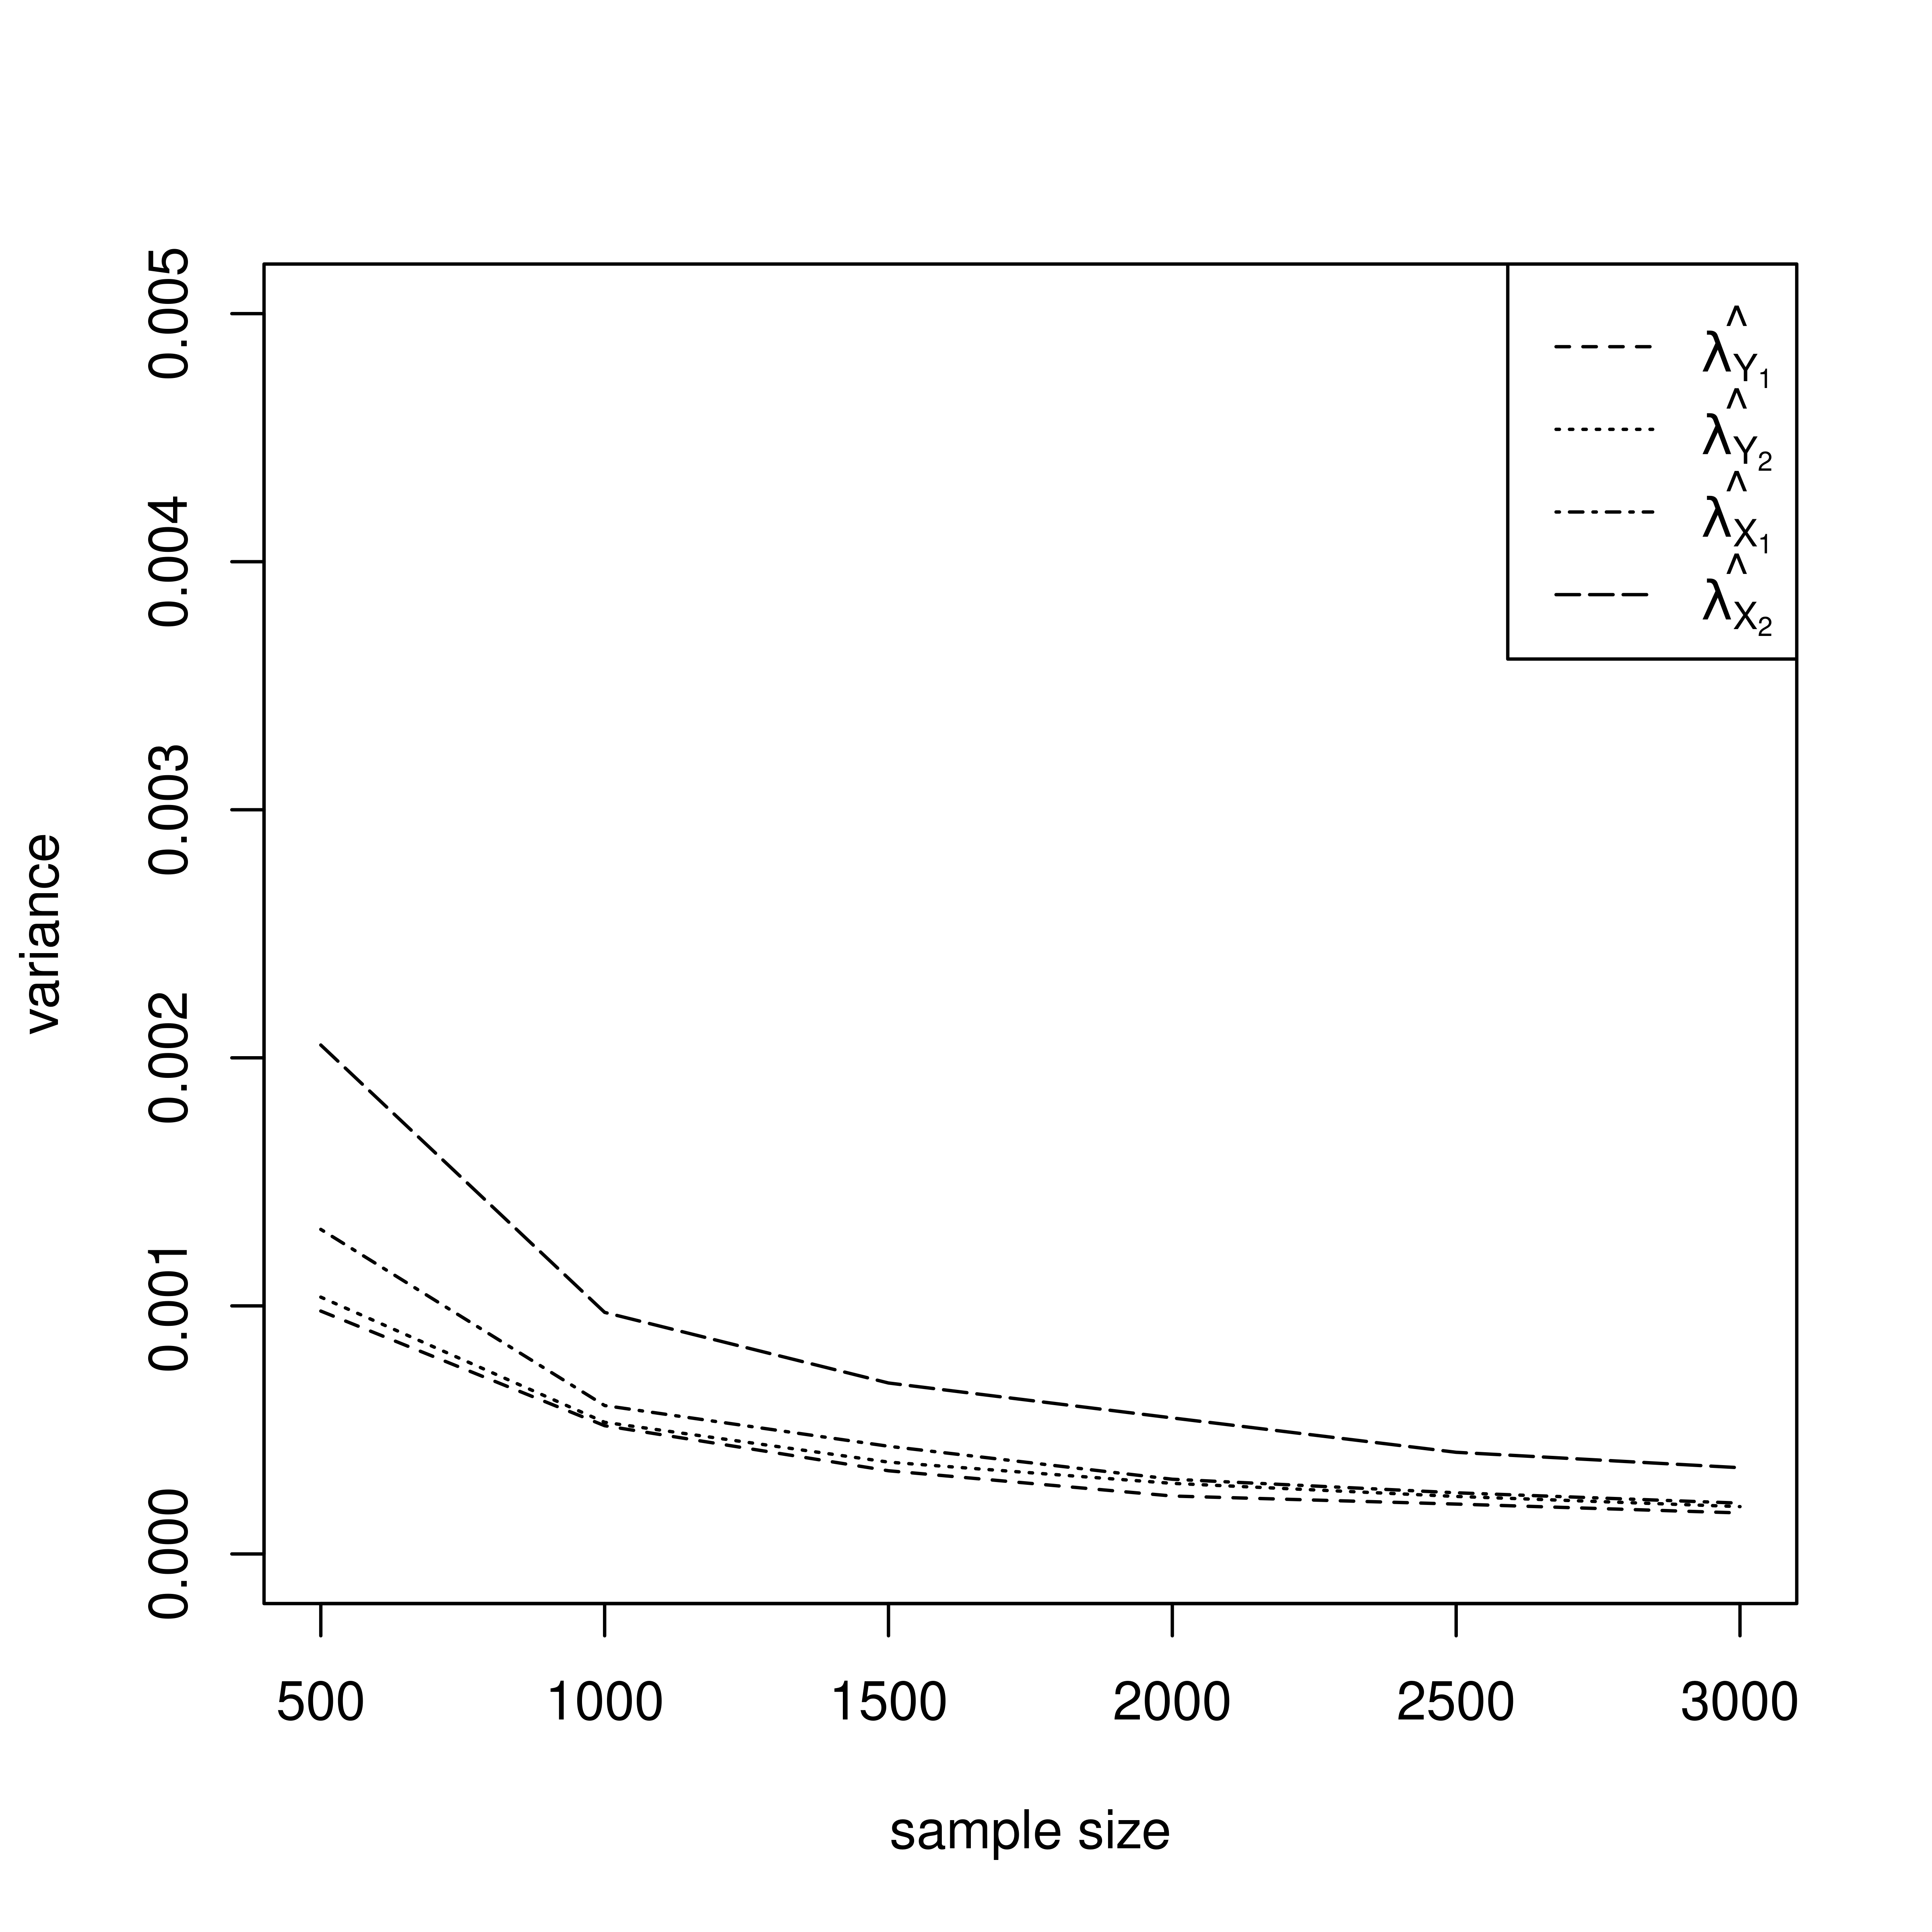
\includegraphics[width=\textwidth]{fig/var_uneq_discrim_high.png}
      \caption{Variance}
    \end{subfigure}
    \caption{Bias and variance of the LS estimator}
    \label{fig:ls_bias_var}
  \end{figure}
  The estimator appears unbiased across sample sizes. Furthermore, the variance
  of the estimator decreases toward 0 as the sample size increases. While not a
  formal proof, this result suggests the LS estimator is likely a consistent
  estimator and has a good performance.

  \subsection{Comparison of the BLP and the CUBLP}
  We analytically showed how the BLP is biased conditional on the true score $S$
  and the unbiasedness of the CUBLP in previous sections. Here, we empirically
  verify the results using a simulation. The data are generated in the same
  fashion as described in the previous simulation. For the same data set $\bW$,
  we computed both the BLP and the CUBLP. The results are in Figure~\ref{fig:prediction}.
  \begin{figure}[t]
     \centering{}
     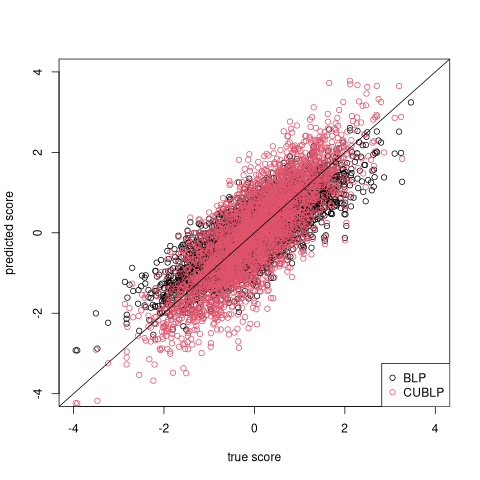
\includegraphics[scale=0.55]{fig/prediction.png}
     \caption{BLP vs. CUBLP in predicting true score.}
     \label{fig:prediction}
  \end{figure}
  Consistent with the analytical results, there are not much noticeable
  difference between the two estimators if the true score is close to $0$, and
  both are unbiased. However, as the true score moves away from $0$ toward
  either extreme, the BLP starts to show biased predictions. For higher
  performers, the BLP underestimates on average. On the other hand, it
  overestimates on average for lower performers.

  \section{Real data analysis}
  To demonstrate the utilities of the proposed method, we analyze a real data
  set. As part of the speaking section of an English language proficiency test,
  students are asked to repeat what they have heard. The sentences vary in
  lengths and may situate in different scenarios such as presentations and
  campus tours. Each recorded response is scored by two different trained raters
  according to the rubric. The rating scale is from 0 to 5 with 5 being the
  highest possible. The two scores may agree or differ. In addition to the human
  raters, the \textit{SpeechRater}\texttrademark system of Educational Testing
  Service (ETS), an automated scoring system for non-native speech, is used to
  evaluate the recorded response. The system provides features related
  to different dimensions of a speech. For the purpose of this demonstration,
  we computed composite scores on accuracy, pronunciation, fluency, and rhythm
  by aggregating the extracted features. These composite scores are standardized
  to have means of 0 and variances of 1. 

  There is a total number of 7690 observations. Since the raters are randomly
  assigned for each observation, we do not have any reason to believe the two
  human scores have a significant difference in discrimination. Therefore, we
  assume the loadings for the two human scores are equal. The estimated CUBLP
  coefficients, BLP coefficients, and the loadings are in Table~
  \ref{tab:coefs_real_data}.
  \begin{table}[!htbp]
  \vspace*{2em}
    \centering\caption{Parameter estimates and predictor coefficients} 
    \label{tab:coefs_real_data} 
  \begin{tabular}{@{\extracolsep{5pt}} cccc} 
  \\[-1.8ex]\hline 
  \hline \\[-1.8ex] 
   & CUBLP & BLP & $\hat{\blambda}$ \\ 
  \hline \\[-1.8ex] 
  rating 1 & $0.456$ & $0.433$ & $0.944$ \\ 
  rating 2 & $0.452$ & $0.430$ & $0.944$ \\ 
  accuracy & $0.144$ & $0.137$ & $0.839$ \\ 
  pronunciation & $0.009$ & $0.009$ & $0.333$ \\ 
  fluency & $0.017$ & $0.016$ & $0.400$ \\ 
  rhythm & $0.025$ & $0.024$ & $0.468$ \\ 
  \hline \\[-1.8ex] 
  \end{tabular} 
  \end{table}
  In this example, the estimated loadings on both human scores and accuracy
  dimension are quite large. As a result, a large amount of observed covariance
  can be explained well by the latent true score. In fact, plug in the
  estimators, the ratio $\hat{\blambda^\top} \hat{\bsigma_{\bW}^{-1}}
  \hat{\blambda} = 0.95$. Therefore, the conditional bias of the BLP estimator
  would not be too large. This is reflected by the closeness of the estimated
  CUBLP coefficients an the BLP coefficients. But, compared to the CUBLP
  estimator, we still see the BLP underestimates for higher performers and
  overestimates for lower performers (see Figure~\ref{fig:comp_real_data}).
  \begin{figure}[t]
    \centering
    \begin{subfigure}[b]{0.45\textwidth}
      \centering
      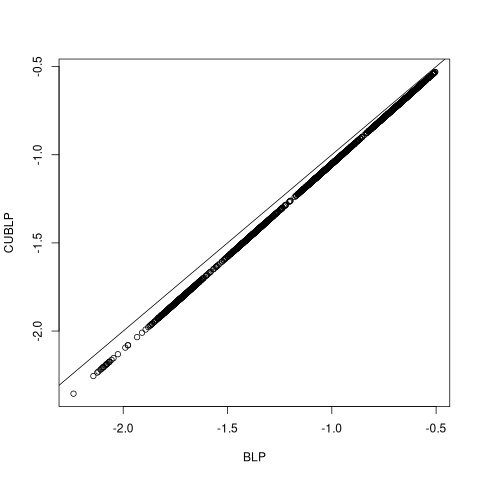
\includegraphics[width=\textwidth]{fig/lower_S.png}
      \caption{Lower performers}
    \end{subfigure}
    \begin{subfigure}[b]{0.45\textwidth}
      \centering
      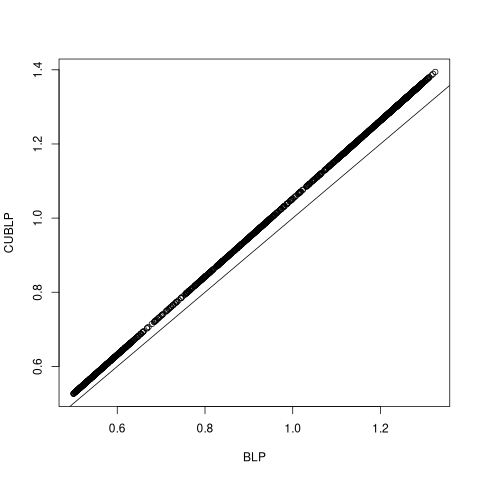
\includegraphics[width=\textwidth]{fig/higher_S.png}
      \caption{Higher performers}
    \end{subfigure}
    \caption{Comparison between the BLP and CUBLP}
    \label{fig:comp_real_data}
  \end{figure}

  \section{Discussion}
  The improved technology enables the collection of more information related to
  the construct of interest from different sources. While it is tempting to
  combine these additional information with the traditional assessment data in
  making inferences on students' proficiency, researchers should be careful so
  that no systematic bias is introduced. The proposed CUBLP method addresses
  one specific source of bias - the algorithmic bias. The method does not
  generally rely on parametric distributional assumption. Consequently, it can
  be applied to a wide range of data and applications.

  The current paper focuses on developing the CUBLP estimator. However, the
  uncertainty of the estimator has not been investigated. Finding the variance
  or the asymptotic variance of the estimator should be an important topic of
  future research.




  \printbibliography
  



\end{document}